%\documentclass[english,10pt]{beamer}
\documentclass[english,10pt,handout]{beamer}






 
%\usepackage{mathptmx}
%\renewcommand{\sfdefault}{lmss}
\usepackage[T1]{fontenc}
%\usepackage[latin9]{inputenc}
\usepackage[utf8]{inputenc}

\synctex=-1

\usefonttheme{professionalfonts}

%\setbeamertemplate{navigation symbols}{}
%\setbeamertemplate{caption}[numbered]


\useinnertheme{rectangles}
%http://tex.stackexchange.com/questions/11168/change-bullet-style-formatting-in-beamer

 \AtBeginDocument{
  \addtolength\abovedisplayskip{-0.4\baselineskip}%
  \addtolength\belowdisplayskip{-0.4\baselineskip}%
}%change the space between text lines and the math formula


\usepackage{pifont}
%Postscript ZipfDingbats font
%the command \ding{number}, will print the specified symbol

\usepackage{fontawesome}
%icon package
\DeclareFontFamily{U}{FontAwesomeOne}{}
\DeclareFontShape{U}{FontAwesomeOne}{m}{n}{<-> FontAwesome--fontawesomeone}{}
\DeclareRobustCommand\FAone{\fontencoding{U}\fontfamily{FontAwesomeOne}\fontseries{m}\fontshape{n}\selectfont}
\DeclareFontFamily{U}{FontAwesomeTwo}{}
\DeclareFontShape{U}{FontAwesomeTwo}{m}{n}{<-> FontAwesome--fontawesometwo}{}
\DeclareRobustCommand\FAtwo{\fontencoding{U}\fontfamily{FontAwesomeTwo}\fontseries{m}\fontshape{n}\selectfont}
\DeclareFontFamily{U}{FontAwesomeThree}{}
\DeclareFontShape{U}{FontAwesomeThree}{m}{n}{<-> FontAwesome--fontawesomethree}{}
\DeclareRobustCommand\FAthree{\fontencoding{U}\fontfamily{FontAwesomeThree}\fontseries{m}\fontshape{n}\selectfont}

%ftp://ftp.dante.de/tex-archive/fonts/fontawesome/doc/fontawesome.pdf
%http://tug.ctan.org/info/symbols/comprehensive/symbols-a4.pdf


\usepackage{amsmath,amssymb,amsfonts,bm,mathrsfs,mathtools}

\usepackage{tikzsymbols}
%\usepackage[tikz]{bclogo}



\usepackage{perpage}
\MakePerPage{footnote} %reset for each page
%\renewcommand{\thefootnote}{\fnsymbol{footnote}} %use symbol, limit less than 9 symbols



%%%% HIGHTLIGHT  and annotation &=%%%%%%%%
\usepackage{color,xcolor}
 \usepackage{todonotes}

\usepackage[normalem]{ulem}

\usepackage[many]{tcolorbox}

\tcbset{fonttitle=\scriptsize}
\tcbset{highlight math style={enhanced,
  colframe=red!40!black,colback=yellow!20!white,arc=2pt,boxrule=.2pt,
  }}
  \newtcbox{\otherbox}[1][]{nobeforeafter,math upper,tcbox raise base,
enhanced,frame hidden,boxrule=0pt,interior style={top color=green!10!white,
bottom color=green!10!white,middle color=green!50!yellow},
fuzzy halo=1pt with green,#1}
%%\tcbhighmath{math here}
%% \otherbox{math here}



%%%%% HIGHLIGHT %%%%%%
\newcommand{\hb}[1]{{\color{blue}{#1}}}
%\noindent\rule{\textwidth}{.5pt}

%:
\usepackage{soul}

\newcommand\hcancel[2][black]{\setbox0=\hbox{$#2$}%
\rlap{\raisebox{.45\ht0}{\textcolor{#1}{\rule{\wd0}{1pt}}}}#2}
%cross to delete

\newcommand{\mcb}[2]{\colorbox{#1}{$\displaystyle #2$}}
%highlight math

\newcommand{\hlfancy}[2]{\sethlcolor{#1}\hl{#2}}
%specified color , for\hl

\newcommand\myhl{\bgroup\markoverwith
  {\textcolor{yellow}{\rule[-.5ex]{2pt}{2.5ex}}}\ULon}



\mode<presentation>{ \usetheme{boxes} }

%write Matlab code
\usepackage{listings}
 \definecolor{dkgreen}{rgb}{0,0.6,0}
\definecolor{gray}{rgb}{0.5,0.5,0.5}
\definecolor{mauve}{rgb}{0.58,0,0.82}
\lstset{frame=tb,
  language=Matlab,
  aboveskip=3mm,
  belowskip=3mm,
  showstringspaces=false,
  columns=flexible,
  basicstyle={\small\ttfamily},
  numbers=none,
  numberstyle=\tiny\color{gray},
  keywordstyle=\color{blue},
  commentstyle=\color{dkgreen},
  stringstyle=\color{mauve},
  breaklines=true,
  breakatwhitespace=true
  tabsize=3
}

\usepackage[lastexercise]{exercise}

\newtheorem{ex}{Exercise}
\newtheorem{property}{Property}
\newtheorem{ag}{Algorithm}
\newtheorem{remark}{Remark}
\newtheorem{den}{definition}
\newtheorem{assumption}{Assumption}


\usepackage[nosolutionfiles]{answers}
\Newassociation{sol}{Solution}{ans}



\usepackage{empheq}
\usepackage{comment}
%\usepackage{lscape}
\usepackage{multirow}
\usepackage{url,hyperref}

\hypersetup{
 %   bookmarks=true,         % show bookmarks bar?
    unicode=false,          % non-Latin characters in Acrobat's bookmarks
    pdftoolbar=true,        % show Acrobat's toolbar?
    pdfmenubar=true,        % show Acrobat's menu?
    pdffitwindow=false,     % window fit to page when opened
    pdfstartview={FitH},    % fits the width of the page to the window
    pdftitle={My title},    % title
    pdfauthor={Author},     % author
    pdfsubject={Subject},   % subject of the document
    pdfcreator={Creator},   % creator of the document
    pdfproducer={Producer}, % producer of the document
    pdfkeywords={keyword1} {key2} {key3}, % list of keywords
    pdfnewwindow=true,      % links in new window
    colorlinks=true,       % false: boxed links; true: colored links
    linkcolor=red,          % color of internal links (change box color with linkbordercolor)
    citecolor=green,        % color of links to bibliography
    filecolor=magenta,      % color of file links
    urlcolor=cyan           % color of external links
}


\usepackage{subfigure,epsfig,graphicx,graphics}

\DeclareGraphicsRule{.tif}{png}{.png}{`convert #1 `dirname #1`/`basename #1 .tif`.png}
   \DeclareGraphicsExtensions{.pdf}




\newcommand{\hw}{ {\underline{\tt Homework }} }
\newcommand{\hws}{ {\underline{\tt Homework$\star$}} }
\newcommand{\optional}{ {\it optional} }

\newcommand{\MATLAB}{ \texttt{MATLAB}}
\newcommand{\python}{ \texttt{python}}
\newcommand{\Rlang}{ \texttt{R}}
\newcommand{\SAS}{ \texttt{SAS}}
\newcommand{\MC}{Markov Chain}


\newcommand{\tm}{transition matrix}
\newcommand{\rv}{random variable}
\newcommand{\spl} {supervised learning }
 

\newcommand{\dis}{\underline{\tt discussion}: }
\newcommand{\pri}{\underline{\tt principle}: }




\newcommand{\bq}{\scalebox{6}{\textbf{?} }}
\newcommand{\sq}{\scalebox{2}{\textbf{?} }}
\newcommand{\ck} {  {\scalebox{0.8} {\Interval}   } }

\newcommand{\eps}{\varepsilon}
\newcommand{\To}{\longrightarrow}

% 
\newcommand{\Dcal}{\mathtt{D}}
\newcommand{\Hcal}{\mathcal{H}}
\newcommand{\Ecal}{\mathcal{E}}
\newcommand{\Xcal}{\mathcal{X}}
\newcommand{\Ycal}{\mathcal{Y}}
\newcommand{\Zcal}{\mathcal{Z}}

%%Calculus 

\renewcommand{\d}{\ensuremath{\mathrm{d}}}
\newcommand{\dt}{ \ensuremath{\mathrm{d} t } }
\newcommand{\dx}{ \ensuremath{\mathrm{d} x} }
\newcommand{\dy}{ \ensuremath{\mathrm{d} y } }

%indicator function
\newcommand{\indf}{ \ensuremath{\mathbf{1} } }



%probability
\newcommand{\p}{ \mathbb{P}}
\newcommand{\prob}{{\Pr}}
\newcommand{\PP}{\mbox{PP}}%Poisson process
%condition prob
\newcommand{\cPr}[2]{{\Pr\left(#1\mid #2\right)}}

\newcommand{\FF}{{\mathbb{F}}}

\newcommand{\e}{ \operatorname{\mathbb E}}
\newcommand{\Var}{\operatorname{\mathbb{V} }}
\newcommand{\var}{\operatorname{\text{Var} }}
\newcommand{\MSE}{\operatorname{\text{MSE} }}

\newcommand{\Std}{\operatorname{std}}
\newcommand{\Cov}{\operatorname{cov}}

%Matrix  %mathbf
\newcommand{\Pb}{{\mathbf{P}}}
\newcommand{\Qb}{{\mathbf{Q}}}
\newcommand{\Mb}{{\mathbf{M}}}
\newcommand{\cb}{\mathbf{c}}
\newcommand{\bb}{{\mathbf{b}}}

\newcommand{\Tb}{\mathbf{T}}

\newcommand{\Wb}{\mathbf{W}}
\newcommand{\wb}{\mathbf{w}}
\newcommand{\Xb}{\mathbf{X}}

\newcommand{\xb}{\mathbf{x}}

\newcommand{\Wtn}{\mathbb{W}}
\newcommand{\btn}{\mathbf{b}}



\newcommand{\eye}{{\mathbf{I}}}
%identity matrix
\newcommand{\onem}{{\mathbb{1}}}
\newcommand{\idor}{\mathbf{1}}
\newcommand{\ii}{\mathbf{i}}
%imaginary symbol

\usepackage{tikz}

%State number
\newcommand{\snum}[1]{ \raisebox{.5pt}{\textcircled{\raisebox{-.9pt} {#1}}}}

 \usetikzlibrary{arrows}
\usetikzlibrary{shapes}

%\newcommand{\snum}[1]{%
 % \tikz[baseline=(char.base)]\node[anchor=south west, draw,rectangle, rounded corners, inner sep=1.4pt, minimum size=5mm,
   % text height=1.3mm](char){\ensuremath{#1}} ;}

\newcommand*\circled[1]{\tikz[baseline=(char.base)]{
            \node[shape=circle,draw,inner sep=.4pt] (char) {#1};}}


%real number
\newcommand{\Real}{{\mathbb{R}}}
%integer
\newcommand{\ZZ}{\mathbb{Z}}
%positive integer
\newcommand{\NN}{\mathbb{N}}



\newcommand{\inpd}[2]{\left\langle #1, #2 \right\rangle}
\newcommand{\abs}[1]{\left\vert#1\right\vert}
\newcommand{\norm}[1]{\left\|#1\right\|}
\newcommand{\wt}[1]{{\widetilde{#1}}}
\newcommand{\set}[1]{\left\{#1\right\}}
\newcommand{\partiald}[2]{  \frac{\partial #1 }{\partial #2}}



\newcommand{\ie}{{\it{i.e.}}}



\newcommand{\transpose}{\textsf{T}} % or, \intercal
\newcommand{\diag}{\textsf{diag}}
\newcommand{\tr}{{\textsf{T}}}
\newcommand{\rt}{{\textbf{r}}}

\DeclareMathOperator{\trace}{Trace}


\newcommand{\argmin}{ \operatornamewithlimits{argmin} }
\newcommand{\argmax}{ \operatornamewithlimits{argmax} }




\def\biz{\begin{itemize} }
\def\bizp{\begin{itemize}[<+->] }
\def\eiz{\end{itemize}}


\def\bfm{\begin{frame}}
\def\efm{\end{frame}}

\def\bena{\begin{enumerate}[<+-| alert@+>]}
\def\ben{\begin{enumerate}}
\def\een{\end{enumerate}}


\def\bbk{\begin{block} }
\def\ebk{\end{block}}






\makeatletter
%%%%%%%%%%%%%%%%%%%%%%%%%%%%%% Textclass specific LaTeX commands.
 % this default might be overridden by plain title style

%%%%%%%%%%%%%%%%%%%%%%%%%%%%%% User specified LaTeX commands.
%\usetheme{Warsaw}
\usetheme{Boadilla}
% or ...



%\setbeamertemplate{footline}[text line]{} % makes the footer EMPTY
%\setbeamertemplate{footline}[page number]{} % makes the footer EMPTY

%\usecolortheme{orchid} %not use is better 

\setbeamertemplate{footline}[text line]{%
  \parbox{\linewidth}{\vspace*{-2pt}Xiang Zhou\hfill CityU\hfill \insertpagenumber}}
%\setbeamertemplate{navigation symbols}{}

%\setbeamercovered{transparent}
% or whatever (possibly just delete it)


%\usepackage{babel}
\makeatother



 %
%\addtobeamertemplate{frametitle}{}{%
%\begin{tikzpicture}[remember picture,overlay]
%\node[anchor=south east,yshift=2pt] at (current page.south east) {
\includegraphics[height=0.6cm]{CityU_Logo_Basic_Signature.eps}};
%\end{tikzpicture}}
%

\beamerdefaultoverlayspecification{<+->}
%the presentation acts as though a \pause command has been inserted between every two bullets, without the actual need to write \pause after each item.



\title{MA4546: Introduction to Stochastic Process}

\author{
\includegraphics[height=1.1cm,width=2.2cm]{CityU_Logo_Basic_Signature.eps}
\\ $\ $ \\
Xiang Zhou  \\ $\ $ \\
}
\institute[]{Department of Mathematics
}

\date[]{}
%{2016-2017, Semester A}



\begin{document}
 
 


\maketitle
 




\frame{
\frametitle{Grading Policy}

\begin{itemize}

\item closed-book final exam: 70\%; 

\item  coursework: 30\%

\begin{itemize}
\item 10\% :  one midterm test 
\item 10\% :  average of two best marks from several in-class quizzes.
\item 
10\% : take-home assignments   (\hw.  Marked with $\star$ is optional)
\end{itemize}
\end{itemize}

\medskip 
{\bf penalty  for late submission of homework}:
{\small (usually two weeks are given for each assignment
and the solution are released online within 1-2 days after submission deadline.)}
\biz
\item   before  the release of answers:     10\% subtraction from you original score.
\item 
after  the release of answers:     50\% subtraction from your original score.
\eiz

\medskip

{\bf No makeup for midterm test or quiz.
}
For the justified  and approved medical reason for the absence of the midterm test,
10\% part  may be added to 70\% for  the final test.


}


\frame{%{Outline}

{\bf TEXTBOOK}: 

{\tt   Introduction to modeling and analysis of stochastic systems} [CityU Library holds electronic resource]  \par
author : Kulkarni, Vidyadhar G.
New York : Springer Science+Business Media, LLC, 2011.
2nd ed.
\\
\medskip
{\bf reference book (optional)}
{\tt  
Understanding Markov Chains: Examples and Applications}
author : Privault,  Nicolas 
Springer Undergraduate Mathematics Series. 2013
(ebook link:  \url{http://link.springer.com/book/10.1007/978-981-4451-51-2})
\bigskip 
\pause

{\bf Our Plan}

\biz
\item Chapter 1:   Review of Probability  (1w)
\item Chapter 2:   Discrete-Time Markov Models (4$\sim$5 w)
\item Chapter 3:   Poisson Processes (2.5w)
 \item Chapter 4*:  Continuous-Time Markov Models (2.5w)
 \item Chapter 7*:  Brownian Motion (2w)

{\footnotesize *: partial coverage of the textbook}
\eiz

}


\frame{{Stochastic process is  time-dependent   description (process) of  random phenomena.}
\begin{figure}
% \includegraphics[width=0.8\textwidth]{BruceLee.jpg}
% \caption{ \bf Knowledge is Power. If you do not apply it, it is {\it other's} power}
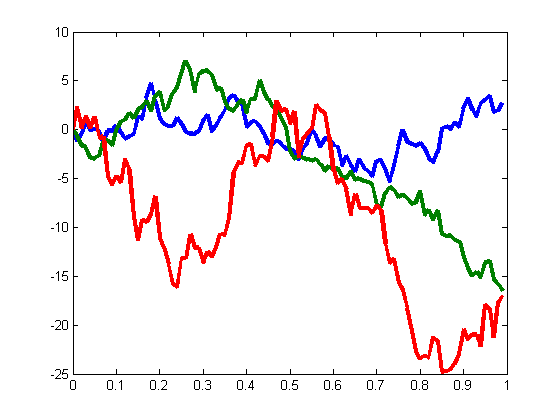
\includegraphics[width=0.5\textwidth]{Wiener.png}
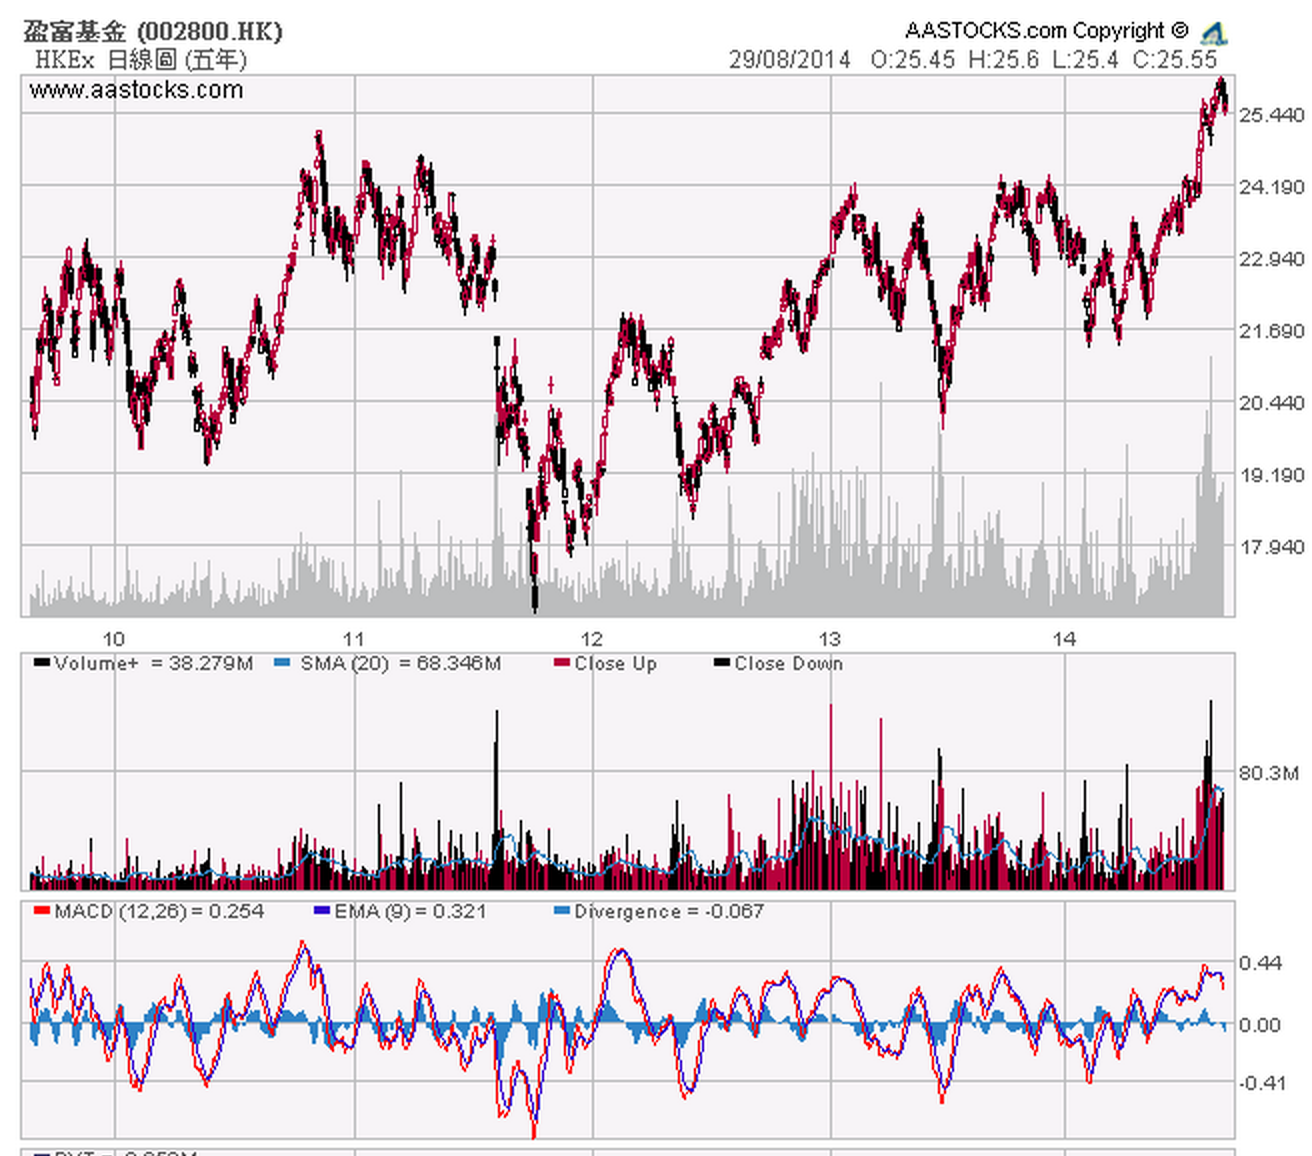
\includegraphics[width=0.5\textwidth]{stock.png}
%\caption{ }
 \end{figure}
}


\frame{ {Deterministic vs Stochastic, which one do you like ?}
\biz
\item  Terminology :   {\it  stochastic,  \pause random,  probability, chance, uncertainty, unpredictable  }
\pause
\item {flip coins:  HTTTHTHHTHHTHHT ...}
\item {gambling:   hong kong horse racing, max six, ... }
%\pause
%\includegraphics[scale=0.6]{maxsix.png}
\item {thermal fluctuation (statistical physics):  
temperature =  randomness in a large population of atoms = entropy = complexity of the microscopic world }
\item {incomplete information:  weather predication;  financial market;  risk analysis }
\item{application:  financial engineering, statistical physics, weather forecast,  risk analysis, statistics,  geology, data sciences, }
\eiz 
\pause{What is ``probability'' \bq
}


}


\frame{
\frametitle{Chapter 1,  (part i)  Review of Probability Theory}
%\only<1|handout:0>{
%\begin{figure}
% 
\includegraphics[scale=0.2]{WenGuZhiXin.jpg}
% \caption{ {\bf Confucius: } ``He who by reviewing the old can gain knowledge of the new and is fit to be a teacher." }
% \end{figure}
% }

}


\begin{frame}
\frametitle{Probability space:  Kolmogorov's axioms  }
A probability model is a  triplet ($\Omega, \mathcal{F},\p$) ({\it Andrey Kolmogorov 1930s }):
\begin{itemize}
\item sample space: $\Omega$.
\item set of events of interest: $\mathcal{F}\subset2^{\Omega}$ (all subsets of $\Omega$).
\item probability (measure) of these events: $\p$ : $\mathcal{F}\to[0,1]$, which satisfies 

\pause
\begin{itemize}
\item $\p(\Omega)=1,\prob(\emptyset)=0$
\item \textbf{countable additivity}: For any countable collection $\left\{ A_{i}\right\} ,i=1,2,3,\cdots,$
of pairwise disjoint sets ($A_{i}\cap A_{j}=\emptyset$ if $i\neq j$
):
\[
\prob(\underset{i}{\cup}A_{i})=\sum_{i}\prob(A_{i})
\]
\end{itemize}
\end{itemize}





\pause
$\mathcal{F}$, a set
of some subsets of $\Omega$ on which $\p$ is defines, satisfies
\begin{itemize}
\item $\Omega\in\mathcal{F}$
\item closed under complements: if $A\in\mathcal{F},$then also $(A^c)\in\mathcal{F}$
\item closed uner \textbf{countable unions: }if $ $$\left\{ A_{i}\right\} \in\mathcal{F}$,
then also $(\underset{i}{\cup}A_{i})\in\mathcal{F}$ .
\end{itemize}
\pause 
The collection of sets satisfying the above conditions is called a $\sigma$-algebra.
\end{frame}




\begin{frame}
\frametitle{Basics of Probability Theory}
\begin{itemize}

\item 
{\bf De Morgan's laws}
\[ (\cup_i A_i)^c = \cap_i (A_i^c), \qquad 
(\cap_i A_i)^c = \cup_i (A_i^c)\]

\item 
 {\bf Inclusion-Exclusion Principle}
\[
\begin{split}
\p\left(\cup_{i=1}^n A_i \right) = \sum_{i=1}^n \p(A_i)
& -\sum_{i<j} P(A_iA_j)
 + \sum_{i<j<k} P(A_iA_jA_k)
 \\& \cdots 
 (-1)^{n+1} P\left(\cap_{i=1}^n A_i\right)
 \end{split}\]
 
example:
\\
$n=2$, $\p(A\cup B)=\p(A)+\p(B)-\p(AB)$ 
\[
\begin{split}
n=3, \quad &\p(A\cup B \cup C)=\p(A)+\p(B\cup C)-\p(A(B\cup C)) \\
&=\p(A)+\p(B\cup C)-\p((AB) \cup  (AC)) \\
&=\p(A)+\p(B) + \p(C)-\p(BC)-
\bigg(\p(AB)  + \p(AC) - \p(ABC) \bigg)\\
&=\p(A)+\p(B) + \p(C)-\p(BC)-\p(AB)  - \p(AC)+ \p(ABC).
\end{split}
\]
\item 
Given a subset $A\subset \Omega$, 
define an {\bf  indicator function}  $\Omega \to \{0,1\}$
\[
1_{A}(\omega)= 
\begin{cases}1, & \mbox{if } \omega \in A \\
0, &\mbox{if } \omega \notin A 
\end{cases}
\]

%
%\item 
%{{\bf continuity} of $\p$}
%
%
%Let  $\{B_n\}$ be a countable collection sets of $\Omega$   such that $B_{n}\supset B_{n+1}$ for all $n$, and
%let $B=\underset{n\geq 1}{\cap} B_n=\{\omega\in \Omega:  \omega \in B_n \mbox{ for all } n=1,2,\cdots\}$, 
%which is usually denoted by $B=\lim_n B_n$, then
%\[\lim_n \p(B_n) = \p(B)=\p(\lim_n B_n)\]
%
%\item {$\limsup$ and $\liminf$} ({\it optional material})
%
%For any sequence of sets $\{A_m\}$,  then $B_n=\underset{m\geq n}{\cup}A_m$ satisfies the above condition.
%The limit $B=\lim B_n = \underset{n\geq 1}{\bigcap}\underset{m\geq n}{\bigcup}A_m $ is denoted as 
%$\limsup_m  A_m$.
%\[\omega \in  \limsup_m  A_m  \iff  \omega \in  A_m \mbox{ for infinitely many } m.\]
\end{itemize}


\end{frame}
  

\begin{frame}
\frametitle{Random variable and its distribution}
\begin{itemize}[<+->]
\item
A random variable (r.v.) $X$ is a function  $X: \Omega \to  \Real =(-\infty,\infty)$
\footnote{strictly speaking,   $X$  is a ``measurable" function from the triplet $(\Omega,\mathcal{F},\p)$ to
 $ ((-\infty,\infty), \mathcal{B})$ such that $X^{-1}(E)\triangleq\{\omega\in \Omega: X(\omega)\in E\} \in \mathcal{F}$
for all $E\in \mathcal{B}$, where the Borel set $\mathcal{B}$
is the smallest $\sigma$-algebra including all open intervals of $(-\infty,\infty)$.}

\item notation convention : capitalized letters for r.v.s; low case letters for specific numerical values. 

\item for each set   $A\in \mathcal{B}$
\[\p(  \{X\in A \} ) \triangleq \p(\{\omega\in\Omega:  X(\omega)\in A\})=\p(X^{-1}(A))\]
\item 
This induces a new probability measure 
$\FF_X(A)\triangleq\p(X \in A),\ \forall A\in \mathcal{B}$ on $(\Real, \mathcal{B})$, which is the {\em distribution (law)}
of the r.v. $X$.  We have a new probability space $(\Real, \mathcal{B}, \FF_X)$.

\item In particular, for the representative subset $A=(-\infty,x]$, 
we can define
Cumulative Distribution Function (``CDF")
$F(x)=\FF((-\infty,x))=\p(X\leq x)$,
which is also sometimes written as $F_X$ to show the underlying r.v. is $X$.

\item If a Probability Density Function (``PDF") exists, then\footnote{strictly speaking, this integration is Lebesgue integration.}
\[F(x)=\int_{-\infty}^x p(x')dx',\qquad p(x)=F'(x).\]
\end{itemize} 
\end{frame}



\begin{frame}
\frametitle{Functions of Random Variable}
Let $X$ be a random variable and $g$ be a function $\Real\to\Real$. 
Then $Y(\omega)=g(X(\omega))$ is another random variable.
What is the law of $Y$ ? 

\pause
$$\FF_Y = \FF_X \circ g^{-1}$$
because the law of $Y$ is calculated as follows: for any (measurable) event $E\in \mathcal{F}$,
\[
\begin{split}
\FF_Y(E)\triangleq \p(Y\in E)=\p(\{g(X(\omega))\in E \})
\\
=\p(X(\omega)\in g^{-1}(E))=\FF_X(g^{-1}(E))
\end{split}\]
where  $g^{-1}$ is the inverse of $g$ defined as 
\[g^{-1}(A) \triangleq \set{x\in \Real:  g(x)\in A }, ~~\forall A\subset \Real.\]
\pause 

\medskip

{\bf Example}
$Y=X^2$. Then CDF of $Y$ is 
$F_Y(y)=\p(Y\leq y)=\p(X^2\leq y) = F_X(\sqrt{y})-F_X(-\sqrt{y})$
for all $y\geq 0$.
\\

\medskip 
\end{frame}


\begin{frame}{Generalized inverse of CDF and its application}
\biz 
\item 
If   $F$ is the CDF of  a r.v. $X$,
the {\bf quantile function or   generalized inverse} of $F$ is defined as 
$$F^{-}(v) \triangleq \inf\set{x:  F(x) \geq v}.$$

$F^-(0.5)$ is called  the {\em median}.

\item
Let $F$ be  a monotonically nondecreasing function taking value $[0,1]$. 
 Define it generalized inverse  
$$F^{-}(v) = \inf\{x:  F(x) \geq v\}$$
Show that if a random variable $X$ has a uniform distribution $U[0, 1]$, then the CDF of the random variable  $Y\triangleq F^{-}(X)$
is exactly the function  $F$. 

\item {\it proof:}  $\p(Y\leq y)= \p(F^{-}(X)\leq y)=\p(X\leq F(y)) = F(y)$.

\item 


{This fact  is used to generate some random variable using the inverse transform sampling-method.}
\eiz

\pause
{\bf example}
The exponential distribution, $\mbox{Exp}(\lambda)$, has CDF $F(x)=1-e^{-\lambda x}$ for all $x\geq 0$.
So, $F^-(v)=-\frac{1}{\lambda} \log (1-v)$ for all $v\in (0,1)$.
Thus the formula $-\frac{1}{\lambda} \log (1-X)$ will generate $\mbox{Exp}(\lambda)$ random variable,  by generating a uniform distribution random variable $X\sim U(0,1)$ first.

\end{frame}




\begin{frame}
{Moment-generating function}
\biz
\item 
The moment-generating function of a r.v. $X$ is 
\[
{\displaystyle M_{X}(t):=\e \!\left[e^{tX}\right] = \int e^{t x}p_X(x)\! dx,\quad t\in \Real ,} 
\]
wherever this expectation exists. By Taylor expansion,
\[
e^{tX}= 1 + tX + (tX)^2/2 + (tX)^3/3!+\ldots
\]
Then
\[
M_{X}(t):= 1 +  t \e [X] + t^2 \e [X^2] /2 + t^3  \e [X^3]/3!+\ldots
\]
and the $m$-th moment is 
\[\boxed{ \e [X^m] = \frac{d^m M_x (t) }{d t^m}\vert_{t=0}.}\]

\item 
$
M_{X}(-\lambda)=  \int e^{-\lambda x }p_X(x) \! dx$
is just the Laplace transform of the pdf $p_X(x)$.
\eiz

\end{frame}



\begin{frame}
{Characteristic function}
\biz
\item 
The {\bf characteristic  function } of a r.v. $X$ is  a complex-valued function defined by 
($\ii^2 =-1$)
\[
{\displaystyle \varphi_{X}(t):=M_X(\ii t) = \e \!\left[e^{\ii tX}\right] = \int e^{\ii t x}p_X(x)dx,\quad t\in \Real ,} 
\]
wherever this expectation exists. This is the Fourier transform of the pdf $p_X$.
 \item 
 For any two random variables $X_1, X_2$,
$X_1, X_2$ both have the same probability distribution if and only if ${\displaystyle \varphi _{X_{1}}=\varphi _{X_{2}}}$.
The $m$-th moment is 
\[\boxed{ \e [X^m] =(-\ii)^m \frac{d^m 
\varphi_x (t) }{d t^m}\vert_{t=0}.}\]

\item 
 $X_1,\ldots, X_n$ are independent r.v.s,
 {\it if and only if} for  any constants $a_1, \ldots, a_n$,  the characteristic function of the linear combination of the $X_i $'s is
\[
{\displaystyle \varphi _{a_{1}X_{1}+\cdots +a_{n}X_{n}}(t)=\varphi _{X_{1}}(a_{1}t)\cdots \varphi _{X_{n}}(a_{n}t)} \]
\eiz

\end{frame}

\frame { {Normal distribution }
Read Section 7.1 and 7.2 in the TEXTBOOK}

%
%\begin{frame}{more exercises about specific distributions}
%\end{frame}

\begin{frame}
\frametitle{Conditional Probability}
\begin{itemize}[<+->]
\item The conditional probability of an event 
A given that an event B has occurred is
\[\p(A|B ) =\frac{\p(AB)}{\p(B)}\]

\item  Fix $B$, $\p(\cdot\, | B)$ is a {\it probability measure}.
\item  Fix $A$, let $B=\set{\omega}$, then $\p(A|\omega)$ is a {\it random variable} , i.e., a function from $\Omega$  to $[0,1]$.

\end{itemize}
\end{frame}


\begin{frame}
\frametitle{Law of Total Probability and Bayes' rule}

Let $E_1,E_2, E_3, \cdots$ be a set of mutually exclusive and exhaustive events, \ie, 
$$E_i\cap E_j =\emptyset   ~\text{  if } ~  i\neq j,    \mbox{ and}  ~~\cup_{i\geq 1} E_i = \Omega.$$
 Then, for any event $E\in\mathcal{F}$,

 \begin{block}
{Law of Total Probability}
\[\p(E)= \sum_{i\geq 1} \p(E\cap E_i)=\sum_{i\geq 1} \p(E|E_i) \p(E_i)\]
\end{block}
\pause
\begin{block}
{Bayes' Rule}
\[\p(E_i|E)= \frac{ \p(E|E_i) \p(E_i) } {\p(E)} = 
\frac{ \p(E|E_i) \p(E_i) } {\sum_{i\geq 1} \cPr{E}{E_i} \p(E_i)}
\]
\end{block}
\end{frame}

\begin{frame}
\frametitle{Independence}
\begin{itemize}
\item Events A and B are said to be independent of each other if
$\p(AB)=\p(A)\p(B)$.
If $\p(B)>0$, then $\p(A|B)=\p(A)$ if $A$ and $B$ are independent.
\item 
Two r.v.s $X$ and $Y$ are said to be independent of each other if
$\p(X\in A, Y\in B)=\p(X\in A)\p(Y\in B)$ for all set $A$ and $B$, i.e.,
$F_{X,Y}(x,y) = F_X(x) \cdot F_Y(y)$ or 
$p_{X,Y}(x,y)=p_X(x)p_Y(y)$ if pdfs exist.

\pause 
\item 
Mutual(joint) Independence


$\{E_1,E_2,\cdots, E_n\}$ is said to be mutually independent if 
for any subset $S\subset\{1,2,\cdots,n\}$,
\[\p(\underset{i\in S}{\cap} E_i) = \underset{i\in S}{\prod}\p(E_i).\]
i.e.,  {\em any} selection of events from  this collection 
is independent. 

\end{itemize}
\end{frame}





\begin{frame}
\frametitle{Expectation}
\begin{itemize}
\item expectation (with respect to r.v. $X$ with pdf $p_X(x)$):
\[\e(g(X)) = \int g(x) p_X(x)dx\]
\item When we write the notation $\e$, we implicitly assume the underlying distribution $p_X(x)$
is clear to the reader.  It is also sometime to write $\e_X[\cdot]$ to explicitly point out 
the underlying distribution for r.v. $X$.

\item For indicator function, 
$\e(1_A(X))=\p(X\in A)$.
\item Variance 
\pause
\begin{align*}
\Var(g(X))&= \e(g^2(X)) - (\e g(X))^2\\
 &=\int g^2(x)p_X(x)dx - \left(\int g(x)p_X(x)dx\right)^2
\end{align*}
\end{itemize}
\end{frame}
%
%\begin{frame}
%\frametitle{Jensen's inequality and applications}
%
%\begin{block}
%{Jensen's inequality}
%If $\varphi$ is a convex function, then 
%$\varphi(\e(X)) \leq \e(\varphi(X))$.
%\end{block}
%\begin{itemize}[<+->]
%\item {\it Proof}:  let $x_0=\e(X)$, and assume the r.v. $X$ has pdf $p(x)$.
%Since $\varphi(x)$ is convex, then  there is a linear function 
%$l(x)= ax+b$ such that $l(x_0)=\varphi(x_0)$ and $l(x) \leq \varphi(x)$ for all $x$. 
%So $ \e(l(X))\leq \e(\varphi(X)) $. But $\e(l(x))=\e(aX+b)=ax_0+b=l(x_0)=\varphi(\e(X))$.
%
%\item {\bf Exercise:} Show that  (1) $\exp({\e X}) \leq \e (\exp(X))$ for any r.v. $X$;
%(2) $\e(1/X) \e(X) \geq 1$ for any positive r.v. $X$.
%
%\item \hw  If $p$ and $q$ are two pdfs defined on $\Real$, prove that the
%{\bf Kullback-Leibler} divergence(or ``relative entropy") of $q$ from $p$, which is defined as
%\[D(p\|q)\triangleq \int p(x) \log \frac{p(x)}{q(x)}, \]
%is always non-negative. (Hint: consider $\varphi(y)=-\log(y)$)
%\end{itemize}
%\end{frame}

\begin{frame}
\frametitle{ Conditional Expectation}

\begin{itemize}
\item Conditional probability  : $\p(X\in A|Y \in B) = \frac{\p(X\in A, Y\in B)} {\p(Y\in B)}$ for two  r.v.s $X$, $Y$ and two events $A$, $B$.
\item Conditional pdf: 
pdf of $X$ given $Y=y$ is 
\footnote{ $p_{X,Y}(x,y)$ is called  the joint pdf of $(X,Y)$ and
$p_Y(y)\triangleq \int p_{X,Y}(x,y)dx$ is called  the marginal distribution of $Y$. }
\[ p_{X|Y}(x|y)= \frac{p_{X,Y}(x,y)}{p_Y(y)}\]

\item Conditioned expectation given $Y=y$
\[ \e(X|Y=y) = \int x\, p_{X|Y}(x|y) dx \]
View the above as a function $h(y)$, then 
\[\e(X|Y) \triangleq  h(Y) \mbox{ which is a random variable }\]

\item For r.v. $X$ and events $A$,$B$, $\e[X, A|B] $ means $\e[X\cdot1_A|B]=\e [ X \cdot 1_A \cdot 1_B ]/\p(B)$
, which is equal to
$\e[X|A, B] \p(A|B)=\e[ X \cdot 1_A \cdot 1_B ]/\p(AB)  \times ( \p(AB)/\p(B) )$.


%\item Conditional Variance 
%\[\Var(X|Y)=\e[(X - \e(X|Y) )^2|Y]=
%\e(X^2|Y) -(\e(X|Y))^2\]

   

\end{itemize}
\end{frame}


\begin{frame}
\begin{theorem}
\[
\e(g(Y)|Y)=g(Y)\]

\[\e (X g(Y) | Y)=
g(Y) \e(X|Y)\]

\end{theorem}

\bigskip
 \begin{block}{double expectation theorem}
  \[\e(\e(X|Y))=\e(X)\]
\end{block}
$\e(X|Y=y)$ is a function of $y$, say $h(y)$. 
This function $h$ maps any possible value of r.v. $Y$ ( ``information" of $Y$, or
$\sigma$-algebra generated by $Y$)
 into a real number. 
Its expectation (w.r.t to r.v. $Y$) is
\[
\begin{split}
&\e(\e(X|Y))=\e( h(Y)) = \int  h(y)p_Y(y)dy
\\
= & 
\int 
\int x\, p_{X|Y}(x|y) dxp_Y(y)dy=
\int 
\int x\, p_{X,Y}(x, y) dxdy\\  
  =&\int x  p_{X} dx=
  \e(X ) 
\\
  \end{split}
  \]
 


\end{frame}


\frame{{Conditional Expectation as an optimal prediction/projection operator (\optional )
\footnote
{The content marked with ``\optional'' in notes means that these parts are at advance level and will not be covered in any test or quiz
(but possible in \hw). 
}
}


{$\e(X|Y)=h(Y)$: Optimal approximation of $X$ by using  a function of $h(Y)$}

\begin{theorem}
\[\e [ |X-h(Y)|^2] =\min_{g \mbox{ is a function }}  \e (  |X-g(Y)|^2    ) \]
where the function  $h(y)$ is the conditional expectation  $h(y)=\e(X|Y=y)$.
\end{theorem}


{\it Proof {(exercise) }. (hint) first show the orthogonality  $\e[(X-h(Y) )  f(Y) ]=0$ for any function $f$
using the double expectation theorem. Then use the triangular equality
$(x-g)^2=(x-h)^2+(g-h)^2-2(x-h)(g-h)$.}

\bigskip
{This means the conditional expectation is a projection of $X$
onto the linear space of all functions $g(Y)$ in $L_2$ sense.
}


}



\begin{frame}
\frametitle{application (optional)}

\begin{block}
{Variance decomposition formula}
For two r.v.s $X$ and $Y$, 
\[\Var(X) = \e(\Var(X|Y)) + \Var(\e(X|Y))\]
\end{block}
\footnote{If we write explicitly the underling r.v.s for each $\Var$ and $\e$, then the conclusion is 
\[\Var_X(X) = \e_Y(\Var_X(X|Y)) + \Var_Y(\e_X(X|Y)).\]}
\pause
proof:  
Since $\Var(X|Y) = \e(X^2|Y)- (\e(X|Y) )^2$, take expectation on both sides
(a function of $y$) for $Y$, then from double expectation theorem,
\[\e[\Var(X|Y)] = \e[\e(X^2|Y)]- \e[(\e(X|Y) )^2]
=\e (X^2)- \e[h^2(Y)]\]
where $h(y)=\e(X|y)$. On the other hand, 
\begin{align*}
\Var(\e(X|Y))=\Var h(Y)= \e h^2(Y) - (\e h(Y))^2
\\
=\e h^2(Y) - (\e [\e(X|Y)])^2
=\e h^2(Y) - (\e X)^2.
\end{align*}

\end{frame}


\begin{frame}
\frametitle{Random Sums of i.i.d r.v.s }
Let $\{X_n: n =1, 2, 3, \cdots\}$  be a sequence of iid \footnote{independent and identically distributed} random variables with common 
expectation $\e X$ and variance $\Var X$, and let $N$ be a nonnegative integer-valued random variable that is independent of 
$\set{X_n}$. Let $Z=\sum_{n=1}^N X_n$.
Then  
\begin{align*}
\Aboxed{\e (Z) &=\e( X)\,  \e (N)} ~~~\mbox{ (Wald Identity) }
\\
\Aboxed{\Var(Z)&= \e(N)  \Var(X) + (\e(X))^2 \Var(N).}
\end{align*}
\pause
{\it Proof:
Note that from independence between $N$ and $\{X_n\}$, 
\[ \e(Z|N=k)= \e(\sum_{n=1}^N X_n|N=k)=\e(\sum_{n=1}^k X_n|N=k) =\e(\sum_{n=1}^k X_n)= k \e(X) \] 
So, the function $h: k\mapsto \e(Z|N=k) $ is a linear function $h(k)=k \cdot \e(X)$. Therefore, the random variable $\e(Z|N)=h(N) = N\cdot \e(X)$.
By double expectation theorem,  $\e(Z) = \e( \e(Z|N))= \e(h(N)) = \e( X) \e(N)$.

}
\end{frame}

\frame
{
Next, We calculate the mapping $g$ defined as $ k\mapsto \e(Z^2|N=k)$
\[ 
\begin{split}
&\e(Z^2|N=k)= \e ((\sum_{n=1}^k  X_n)^2\,  \vert N=k )\\
&=\e ((\sum_{n=1}^k  X_n)^2 )=\e (\sum_{n=1}^k  X^2_n+ \sum_{1\leq m,n\leq k, m\neq n} X_m X_n   )\\
& =k \e(X_n^2) + (k^2-k) \e(X_n) \e(X_m)\\
&=k^2 (\e X)^2 + k \Var (X).\\
\end{split}
\]
So, $g(k)$ is the quadratic function. $\e(Z^2|N)=g(N)$.
\[
\begin{split}
\Var(Z)&= \e(\e(Z^2|N)) - (\e(Z))^2
=\e(g(N))- (\e N \cdot \e X)^2\\
&=\e[N^2 (\e X)^2  +N\cdot \Var X ]- (\e N \cdot \e X)^2\\ 
&=\e(N^2)\cdot (\e X)^2  +\e N \cdot \Var X- (\e N \cdot \e X)^2\\
&=\Var N \cdot (\e X)^2  +\e N \cdot \Var X.
\end{split}\]
}

%
%\begin{frame}
%\frametitle{A puzzle: Monty Hall Problem (optional)}
%\framesubtitle{View the video on \url{http://www.youtube.com/watch?v=mhlc7peGlGg} }
%
%\pause
%Let be $X$ be the original choice and $Y$ be your final choice.
%Then $X\in\{car, goat\}$ and $\p(X=car)=1/3$, $\p(X=goat)=2/3$.
%
%
%No swapping: $Y=X$ so $\p(Y=car)=\p(X=car) =1/3 $.
%\pause
%
%swapping: 
%from the law of total probability
%\[\begin{split}
%&\p(Y=car) =\p(Y=car, X=car) + \p(Y=car, X=goat)  \\
%=&0 + \p(Y=car| X=goat) \p(X=goat) = \p(X=goat) =2/3.
%\end{split}\]
%by noting the important facts that 
%\[\p(Y=car, X=car)=0 \]
%since there is only {\it one} car  and 
%\[ \p(Y=car | X=goat) =1 \]
%since the host always opens the door for the second goat (which can not be your choice $Y$), 
%and $Y$ is different from $X$, thus 
%$Y$ has to be  the  door  of  car.
%\end{frame}


\frame{{ Chapter 1, (part ii) Random Walk Model }
 \begin{center}
 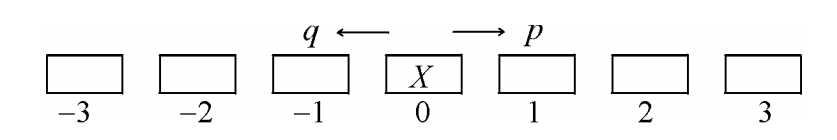
\includegraphics[width=0.86\textwidth]{rw.png}
  \end{center}
  }
  \frame{
  \bizp
  \item
Define  the iid  (Bernoulli) random variable $Z_i = \begin{cases}
 +1,  \quad \mbox{with prob } p  \\
 -1,  \quad \mbox{with prob  } q=1-p .\\
\end{cases}$.

\item What is expectation and variance of $Z_i$ ?

  
\[ \e[Z_i]= -1 \times q + 1 \times  p = p-q := \mu \]
\[
\begin{split} \Var[Z_i]= \e Z^2_i - \mu^2 =  1^2 \times q + 1^2 \times p  -\mu^2
\\
=1-\mu^2=(1+\mu)(1-\mu)=2p*2q=4pq
\end{split}
\]

\item 



 Let $X_0=0$ then  the random walk $(X_n)$ is the random sequence
\[ \boxed{X_n = \sum_{i=1}^n Z_i}\] 
The case of $p=q=1/2$ is called symmetric random walk.
\item 
This is also a gambling model: 
Each bet is $1$ dollar. Win prob is $p$ at each round $n$.
Then $X_n$ is the money at time $n$.
\eiz

}

\frame{
{Distribution of $X_n$}
\[\e X_n = \e (\sum_i Z_i)=\sum_i  \e(Z_i) = n \mu\]
\[\begin{split}
\Var (X_n)& = \e (\sum_i Z_i)^2 - (\e \sum_i Z_i)^2 =
\e\left[ (\sum_i Z_i) (\sum_j Z_j)\right]   -( \sum_i \e Z_i) (\sum_j \e Z_i) 
\\ &=\e  (\sum_i Z_i^2) +
{\color{blue}\e\left[\sum_{i\neq j} Z_i Z_j\right]  }
- \sum_i (\e Z_i) ^2
  -{\color{blue} \sum_{i\neq j } (\e Z_i) ( \e Z_j) }
~~  {\color{blue}\because \set{X_i} \mbox{ indept.}}
\\
&=\sum_i  \left[ \e( Z_i^2)  - (\e Z_i)^2\right]= \sum_i \Var(Z_i) = 4npq
\end{split}\]

\pause
\[ \p(X_1=1)=p, ~ \p(X_1=-1)=q,
\]

\[ \p(X_2=2)=p^2, ~ \p(X_2=0)=2pq,  ~\p(X_2=-2)=q^2,
\]

\[  
  \p(X_3=3)=p^3, ~ \p(X_3=1)=3p^2q,      
~  \p(X_3=-1)=3pq^2,
 ~ \p(X_3=-3)=q^3, 
\]

\[\cdots\]


Yang Hui's Triangle /Pascal Triangle 
}


\frame{{Martingale (\optional)}
\begin{definition}
A stochastic process $M(t)$, where time $t$ is continuous 
($t\in \Real$)
or discrete ($t=0,1,2,\cdots$),
adapted to a filtration $\mathcal{F} = (\mathcal{F}_t:t\in \Real)$ 
is a martingale if for any $t$,
$\e |M(t)|<+\infty$ and for any $s$  and $t$
with $0\leq s<t\leq T$,
\[\e(M(t)|\mathcal{F}_s) = M(s).\]
\end{definition}
\bizp
\item  The filtration $\mathcal{F} = (\mathcal{F}_t: t\in \Real)$  is a stream of information:
the known information up to time $t$ is denoted as $\mathcal{F}_t$.  So, $\mathcal{F}_s \subset \mathcal{F}_t, ~\forall s\leq t$.
\item  adaptive: $M(t) \in \mathcal{F}_t$, i.e., the set $\{M(t)  \leq a\} \in \mathcal{F}_t$ for all
real number  $a$.   
\item   random walk. $\mu:=\e Z_1=p-q=2p-1$. 
Then $(X_n-\mu n)_{n\in \ZZ}$ is a martingale since
\[ \e |X_n-\mu n|\leq \e |X_n| + \mu n \leq  \sum_{i=1}^n \e|Z_1| = \mu n <\infty\]
\begin{align*} 
\e(X_{n+1} -\mu (n+1) \mid Z_n,\cdots,Z_1 ) =  \e(X_{n}   -\mu n + Z_{n+1} - \mu   \mid Z_n,\cdots,Z_1)\\
=\e(X_{n}   -\mu n \mid Z_n ,\cdots,Z_1) + \e(Z_{n+1} - \mu)
= \e(X_{n}   -\mu n \mid Z_n,\cdots,Z_1 ) =X_{n}   -\mu n.
\end{align*}


\eiz

}


\frame{{Predictable process (\optional)}
Let's play the gambling with {\it random} ante:   the stake to bet  at   round $n$ is   $H_n$ dollars. 
Here $(H_n)$ is another stochastic process.
Then the money at time $n$ is 
\[ \boxed{Y_n :=\sum_{i=1}^n  H_i Z_i = \sum_{i=1}^n  H_i (X_i-X_{i-1}).
}\]
 The   natural requirement is that 
$H_n$ is known {\it before} the start of round $n$, i.e.,
\[ H_n \in \mathcal{F}_{n-1} = \text{information of } (Z_1,\cdots,Z_{n-1})
\footnote{We call $(H_n)$ is {\it predictable} w.r.t. $\mathcal{F}=(\mathcal{F}_n)$
if $H_n \in \mathcal{F}_{n-1} $}.\]

\pause
Remark:  
Here we do not need independence of $(H_n: n\in\ZZ)$ and $(Z_n:n\in \ZZ)$.
The   strategy $H_n$ 
can depend on $Z_1,\cdots, Z_{n-1}$,
but not on $Z_n$!

\pause 
Let $p=q$, then  we already know that $(X_n)$ is a martingale.
Show that  $(Y_n)$ is also a martingale w.r.t.  $(\mathcal{F}_n)$ if $  |H_n| <C$ for any $n$;
\pause
\begin{align*}
\e(Y_{n+1}|\mathcal{F}_n)
&=\e(Y_{n}|\mathcal{F}_n)
+ \e( H_{n+1} Z_{n+1}|\mathcal{F}_n)
\\
(\because \text{ predictable }) 
&=\e(Y_{n}|\mathcal{F}_n)
+{\color{red}{H_{n+1}}} \e( Z_{n+1}|\mathcal{F}_n)
\\
&=Y_{n} + H_{n+1} \cdot 0  
=Y_n
\end{align*}
}

\begin{frame}{stochastic integration (\optional)}

\begin{block}{stochastic integration (discrete form)}
{Assume that the stochastic process 
$(X_n)$ is a martingale w.r.t. the filtration $(\mathcal{F}_n)$ and
$(H_n)$ is {\bf predictable} to $(\mathcal{F}_n)$ and $\sup_n |H_n|< \infty$ a.e.
Then,  define 
the stochastic integration 
\[
 \boxed{
 Y_n :=  \sum_{i=1}^n  H_i (X_i-X_{i-1}) 
}~~{\color{cyan}{\sim \int H dX}}
\]
}
\end{block}
\begin{theorem}
   $(Y_n)$ is also a martingale w.r.t.  $(\mathcal{F}_n)$.
\end{theorem}
\pause
{\em Proof: } \vspace{-10pt}
\begin{align*}
\e(Y_{n+1}|\mathcal{F}_n)
&=\e(Y_{n}|\mathcal{F}_n)
+ \e( H_{n+1} (X_{n+1}-X_{n})|\mathcal{F}_n)~~~
\\
(\because \text{ predictable }) 
&=\e(Y_{n}|\mathcal{F}_n)
+{\color{red}{H_{n+1}}} \e(  (X_{n+1}-X_{n})|\mathcal{F}_n)
\\
&=Y_{n} + H_{n+1} (\e(  X_{n+1}\mid \mathcal{F}_n)-X_{n})\\
& = Y_n +H_{n+1}\cdot 0=Y_n
\end{align*}


\end{frame}



\begin{frame}
\frametitle{Exercises \footnote{not \hw,  no need to submit. But you are encouraged to  solve.}}

\begin{enumerate}



\item 
If two r.v.s  $X$ and $Y$ are independent, then
\[p_{X|Y}(x|y) = p_X(x),\qquad \e(X|Y) = \e X.\]



\item
If $\{X_1,X_2,\cdots,X_n\}$ is mutually independent, then
$\Var (\sum_i X_i) = \sum_i \Var(X_i)$

\item Find the moment-generating and characteristic functions
for the following distributions:
Bernoulli distribution $\mathsf{Bern}(p)$, Poisson distribution $\mathsf{Poi}(\lambda)$, 
exponential distribution $\mathsf{Exp}(\lambda)$,  normal distribution $N(\mu,\sigma^2)$.
 \footnote{\href{https://en.wikipedia.org/wiki/Characteristic_function_(probability_theory)}{click for online answer}} 

\item Suppose that 
$X=(X_1,X_2)$ is a two dimensional Gaussian random variable
with mean $\mu=(\mu_1,\mu_2)$ and the covariance matrix
$\Sigma=\left(\begin{smallmatrix}
\sigma^2_1&\rho\sigma_1\sigma_2\\ \rho\sigma_1\sigma_2&\sigma_2^2
\end{smallmatrix}\right )$.
What is the conditional pdf  $p(x_1|x_2)$ of $X_1$ given $X_2=x_2$?
For what value of $\rho$,  $X_1$ and $X_2$ are independent ?
%Verify the variance decomposition theorem for this two Gaussian variables $X_1$ and $X_2$.
%\item  Suppose that $X_1, X_2,X_3$ are three random variables such that 
%the condition distribution of $X_2$ given $X_1=x_1$ is a Gaussian distribution
%with mean $x_1$ and variance $1$ and 
%the condition distribution of $X_3$ given $X_1=x_1, X_2=x_2$ is a Gaussian distribution
%with mean $x_2$ and variance $1$.
%If $X_1$ follows the Gaussian distribution  with mean $0$ and variance $1$,
%what is the joint pdf of $(X_1,X_2,X_3)$? What is the marginal distribution of $X_3$?
%
%(Hint $\p(ABC)=\p(AB|C)\p(C)=\p(A|BC)\p(B|C)\p(C)$)


\item Show that if $(X_t)$ is a martingale, then 
its expectation $\e X_t$ is independent of time $t$. 
%
%
\item For the random walk defined above, find the value 
of a positive number $\sigma$
such that $(X_n-\mu n)^2 -\sigma^2 n $ is a martingale. 

\end{enumerate}
\end{frame}





\end{document}
